\documentclass[12pt]{article}
\usepackage{amssymb,amsmath,amsthm,tikz,multirow,graphicx,xcolor,subfigure}
\usetikzlibrary{calc,arrows}

\begin{document}

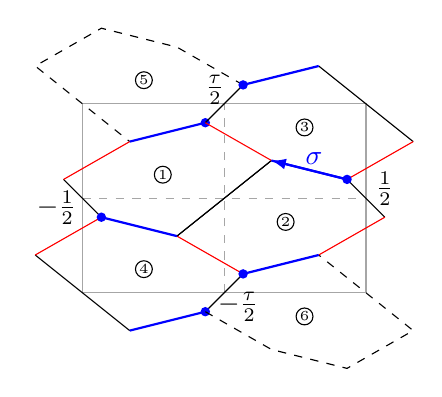
\begin{tikzpicture}[>=latex,scale=0.6]

\draw[gray!70]
	(-3,-2) rectangle (3,2);

\draw[gray!70,dashed]	
	(-3,0) -- (3,0)
	(0,-2) -- (0,2);

\foreach \a in {-1,1}
{
\begin{scope}[scale=\a]

\draw
	(1,0.8) -- (-1,-0.8)
	(2.6,0.4) -- (3.4,-0.4)
	(-0.4,1.6) -- (0.4,2.4)
	(2,2.8) -- (4,1.2);

\draw[dashed]
	(-0.4,-2.4) -- (1,-3.2) -- (2.6,-3.6) -- (4,-2.8) -- (2,-1.2);

\draw[red]
	(1,0.8) -- (-0.4,1.6)
	(2,-1.2) -- (3.4,-0.4)
	(4,1.2) -- (2.6,0.4);

\draw[blue, thick]
	(1,0.8) -- (2.6,0.4)
	(0.4,2.4) -- (2,2.8)
	(0.4,-1.6) -- (2,-1.2);

\fill[blue] 
	(2.6,0.4) circle (0.1)
	(0.4,2.4) circle (0.1)
	(0.4,-1.6) circle (0.1);
	
\end{scope}
}

\draw[blue, thick, <-]
	(1,0.8) -- (2.6,0.4);

\node at (3.4,0.2) {$\frac{1}{2}$};
\node at (-3.55,-0.2) {$-\frac{1}{2}$};
\node at (-0.2,2.3) {$\frac{\tau}{2}$};
\node at (0.3,-2.3) {$-\frac{\tau}{2}$};

\node[blue] at (1.9,0.85) {$\sigma$};

\node[inner sep=0.5, draw, fill=white, shape=circle] at (-1.3,0.5) {\tiny 1};
\node[inner sep=0.5, draw, fill=white, shape=circle] at (-1.7,-1.5) {\tiny 4};
\node[inner sep=0.5, draw, fill=white, shape=circle] at (1.3,-0.5) {\tiny 2};
\node[inner sep=0.5, draw, fill=white, shape=circle] at (1.7,1.5) {\tiny 3};
\node[inner sep=0.5, draw, fill=white, shape=circle] at (-1.7,2.5) {\tiny 5};
\node[inner sep=0.5, draw, fill=white, shape=circle] at (1.7,-2.5) {\tiny 6};
		
\end{tikzpicture}

\end{document}